\section{因子模型的$L_1$范数主成分估计算法研究}

本章继续讨论$L_1$范数主成分分析,重点在于讨论$L_1$主成分分析的求解算法。
$L_1$主成分分析虽然在稳健性上有很大优势,但是其求解需要比$L_2$主成分分析
多得多的时间,在很多场合下限制了它的应用。

在第\ref{chapter3}章的研究中,我们已经重点讨论了优化最小绝对值回归的算法,
注意到交替凸优化算法中包含了最小绝对值回归问题,
本章充分利用第三章得出的结论,尝试将两种算法应用于改良交替凸优化算法。
首先我们阐述改进后算法的具体步骤,之后通过一个模拟实验测试算法的性能。

至此我们已经对问题$P_3$做出了较为深入的讨论,而问题$P_4$同样值得探究,它是$L_1$主成分分析的另一重要研究方向。
我们将介绍一种利用贪婪策略求解$P_4$算法,并通过模拟实验证明算法的有效性。

在第\ref{chapter2}章,我们将交替凸优化算法用于近似因子模型的估计,并且通过实证研究论证了
$L_1$范数主成分分析得出的因子同样适用于宏观经济预测中,并且有良好的预测表现。
本章的最后,我们将求解$P_4$来得到的因子估计量同样在国内主要月度宏观经济数据预测场景下进行了测试,
并给出了一些结论与建议。

\subsection{改进的$L_1$主成分分析交替凸优化算法}
在第\ref{chapter2}章中,我们提出了求解$L_1$主成分分析的交替凸优化算法;
交替凸优化算法的计算量主要集中在\eqref{subpro}和\eqref{subproabs},注意到
在数据服从因子模型的假设下,\eqref{subproabs}是一个最小绝对值回归问题。
因此我们可以尝试使用第\ref{chapter3}章中基于替代变量的估计算法来代替线性规划求解\eqref{subproabs}。

\subsubsection{基于替代变量算法的交替凸优化算法改进}
前文我们已经讨论了一种基于替代变量的估计算法,该算法在求解最小绝对值回归时具有较好的性能提升效果。
在前文已经阐述了该算法的理论基础,注意到\eqref{rho-problem}与\eqref{randomversion}关联起来的前提是线性模型成立。
即需要保证$\mathbb E(Y|\bm{X}^T\bm{\beta})$必须存在。

改写\eqref{subproabs},
\begin{equation}
    \bm a_i = \underset{\bm {\theta}}{\operatorname{arg\ min}} \sum_{j=1}^n |x_{ij} -\bm{\theta}^Tf_j|
\end{equation}
假设数据服从因子模型,可认为$\mathbb E (\bm X|\bm{f})$存在,因此这里\eqref{subproabs}为一最小绝对值回归问题。

下面给出使用基于替代变量的估计算法改进交替凸优化算法的步骤。
\begin{table}[H]%%%%%%开始表格
    \centering%把表居中
    \begin{tabular}{{p{0.9\columnwidth}}}%三个c代表该表一共三列,内容全部居中
    
    \toprule%第一道横线 表头
    {\heiti 算法} {\bf 4.1} 基于替代变量算法改进的交替凸优化算法(ACP-SVN) \\
    \midrule%第二道横线 符号+解释+单位 中间用&隔开
    1.初始化:给出$\bm{A}$,$\bm \Sigma$的初始值$\bm{A}^{(0)}$,这里我们始终采用$L_2$主成分估计的因子载荷矩阵作为初始估计
    ,$\bm \Sigma^{(0)} = \bm I$,(其中$\bm \Sigma$为一对角矩阵,
    $I$为单位矩阵); \\

    2.交替凸优化:对于迭代次数$t = 1, ..., \tau$: \\
    $$p_1:\ \bm F^{(t)} = \underset{\bm F}{\operatorname{arg\ min}} \|\bm X - \bm{A}^{(t-1)}\bm\Sigma^{(t-1)}
    \bm F^{T}\|_{L_1}$$ \\
    $$p_2:\ \bm{A}^{(t)} = \underset{\bm{A}}{\operatorname{arg\ min}} \|\bm X - \bm{A}\bm\Sigma^{(t-1)}{(\bm F^{(t)})}^T \|_{L_1}$$ \\
    $p_1$对应的若干子问题,采用线性规划法求解;$p_2$对应的若干子问题,采用SVN算法求解\\
    \begin{equation*}
        \text{归一化:}\left\{
                    \begin{array}{clr}
                    \bm N_a = diag({(\bm A^{(t)})}^T\bm{A}^{(t)})\\
                    \bm N_f = diag({(\bm F^{(t)})}^T\bm F^{(t)})\\
                    \bm F^{(t)} \leftarrow \bm F^{(t)}\bm N_f^{-1}\\
                    \bm{A}^{(t)}\leftarrow \bm{A}^{(t)}\bm N_a^{-1}\\
                    \bm \Sigma^{(t)} \leftarrow \bm N_a\bm\Sigma^{(t-1)}\bm N_f\\
                    \end{array}
        \right.
    \end{equation*} \\

    3.输出结果:$\bm{A} \leftarrow \bm{A}^{(\tau)}\bm\Sigma^{1/2}$,对$\bm{A}$进行QR分解取正交矩阵得到$\hat{\bm{A}}$;
    $\hat{\bm{F}} \leftarrow \hat{\bm{A}}^T\bm{X}$。
     \\
    \bottomrule%第三道横线
    \end{tabular}
\end{table}%%%%%%结束表格

\subsubsection{基于聚类——迭代拆解算法的交替凸优化算法改进}
上面我们给出了在因子模型假设下交替凸优化的算法改进。
然而对于人脸图像数据的主成分分析、带有噪声的信号数据的主成分分析等情形,
因子模型往往不成立,此时
我们需要寻找更加通用的优化手段。

我们可以尝试使用聚类——迭代拆解算法求解\eqref{subproabs}和\eqref{subpro},
做法是采用聚类——迭代拆解算法对交替每一个子问题进行求解,其余具体步骤同算法2.1。

\subsubsection{数值模拟}
为了对改进后的算法性能进行测试,首先进行数值模拟。这里
我们模拟一个高维的因子模型,用来对比三种方法的求解性能。

令$\bm{f} = (f_1, ..., f_m)$为一$m$维随机变量,服从$N(\bm{0}, \bm{I}_m)$。
根据模型\eqref{orth-factor},为模拟$(X_1, ..., X_p)$,首先随机产生$p\times m$的因子载荷矩阵,
之后产生$\bm{f}$的$n$组随机取值,并求出观测变量的对应观测值矩阵$\bm X $。
最后随机取$10\%$的观测,加上柯西噪声。

取不同的$(m, p, n)$来测试三种算法的性能表现,
我们记录每次取值下算法运行的CPU时间和重构误差(这里就是因子残差)平方的中位数。
部分性能比较结果见\ref{three-l1-pca}
(需要注意本实验是在低功耗便携式计算机上,采用Python脚本测试的。
即使如此,每次实验的时间也和交替凸优化算法的迭代终止条件的选取以及算法实现的方式有很大关联,
本实验的性能结果并不代表交替凸优化算法
标准实现的性能,事实上已经存在一些良好的C++实现,计算性能比我们编写的Python程序要快得多。
另外本实验中$\alpha = 1\times10^{-12}$)
,其中$L_2$主成分分析的因子残差平方中位数也列出。

\begin{table}[H]
    \small
    \centering
    \caption{三种算法的比较结果}
    \label{three-l1-pca}
    \begin{tabular}{@{}cccccccccc@{}}
    \toprule
       &      &     & \multicolumn{2}{c}{ACP} & \multicolumn{2}{c}{ACP-SVN} & \multicolumn{2}{c}{ACP-AID} & PCA-L2   \\ \midrule
    m  & n    & p   & Time     & l2-error     & Time       & l2-error       & Time       & l2-error       & l2-error \\ \midrule
    5  & 1000  & 50  & 47       & 0.0083       & 19         & 0.0115         & 129        & 0.0083         & 0.39     \\
    10 & 1000  & 50  & 68       & 0.0064       & 17         & 0.0096         & 104        & 0.0064         & 0.58     \\
    5  & 5000 & 50  & 119      & 0.0382       & 31         & 0.1232         & 278        & 0.0382         & 1.24     \\
    10 & 5000 & 50  & 107      & 0.0259       & 79         & 0.1352         & 321        & 0.0259         & 0.85     \\
    5  & 5000 & 100 & 689      & 0.0725       & 362        & 0.1480         & 1782       & 0.0725         & 1.26     \\
    10 & 5000 & 100 & 792      & 0.0664       & 510        & 0.2394         & 1440       & 0.0664         & 2.99     \\
    5  & 2000  & 200 & 3567     & 0.0992       & 1135       & 0.4903         & 3290       & 0.0992         & 2.07     \\
    10 & 2000  & 200 & 3893     & 0.1033       & 1650       & 0.5790         & 5033       & 0.1033         & 3.12     \\ \bottomrule
    \end{tabular}
\end{table}

从结果中我们发现,ACP-SVN算法的计算性能优势较为明显,而ACP-AID算法的计算性能表现则相对一般,并没有明显的改进效果。而理论上说,
两者都应该在数据规模较大的情况下有明显的提升,局限于本次实验平台的计算能力,我们把更多的测试留到今后的进一步研究中。

\subsection{求解特征空间$L_1$范数最大化的贪婪算法}

我们已经在第三章中研究了$P_3$,这里我们首选给出问题$P_4$的规范化表述:
\begin{equation}\label{p4}
    P_4: \ \hat{\bm A} = \underset{\bm{A}}{\operatorname{arg \ max}} \| \bm A^T \bm X\|_{L_1}
    = \underset{\bm A}{\operatorname{arg\ max}} 
    \sum_{i=1}^{n}\sum_{k=1}^{m}|\sum_{j=1}^p{a}_{jk}x_{ij}|
     \text{,其中}\bm A^T\bm A = \bm I_m
\end{equation}

这里我们介绍一种求解$P_4$的算法。求解\ref{p4}时,
由于对于不同的$m$,最优$\bm a_j^*$会发生变化,因此想要得出\ref{p4}的全局最优解是非常复杂的。
下面介绍Kwak(2008)提出的一种算法\cite{kwak2008principal},它将问题分解为数个$m=1$的子问题,然后用贪婪策略获得全局解。
该算法直观、简洁并且易于实现。
\subsubsection{求解子问题}

首先考虑$m = 1$的情况,该问题寻找\eqref{m-1}的最优解。
\begin{equation}\label{m-1}
    \bm a^* = \underset{\bm a}{\operatorname{arg\ max}}\| \bm a ^T \bm{X}\|_{L_1}
    = \underset{\bm a}{\operatorname{arg\ max}}\sum_{i=1}^n|\bm a^T\bm x_i|
    \text{,其中}\|\bm a\|_{L_2} = 1
\end{equation}

算法4.2给出了\eqref{m-1}的求解算法。
\begin{table}[H]%%%%%%开始表格
    \centering%把表居中
    \begin{tabular}{{p{0.9\columnwidth}}}%三个c代表该表一共三列,内容全部居中
    
    \toprule%第一道横线 表头
    {\heiti 算法} {\bf 4.2} $m=1$时的$P_4$求解算法\\
    \midrule%第二道横线 符号+解释+单位 中间用&隔开
        初始化:取$\bm a$的任意初始值;$\bm a^{(0)}\leftarrow \bm a^{(0)}/\|\bm a^{(0)}\|_{L_2}$。 \\
        对于$t = 1, ..., \tau$:\\
            1.对所有的$i \in \{1, ..., n\}$,若${(\bm a^{(0)})}^T\bm x_i < 0$,令
            $p_i^{(t)} = -1 $,否则$p_i^{(t)} = 1$ 。\\
            2.令$t \leftarrow t+1$并且$\bm a^{(t)} = \sum_{i=1}^np_i^{(t-1)}\bm x_i$;
            $\bm a^{(t)} \leftarrow \bm a^{(t)}/ \|\bm a^{(t)}\|_{L_2}$ 。\\
            3.检查是否收敛:\\
            1)如果$\bm a^{(t)} \neq \bm a^{(t-1)}$,回到步骤2;\\
            2)若存在某个$i$使得$\bm a^T\bm x_i = 0$,令$\bm a^{(t)} \leftarrow
            (\bm a^{(t)} + \Delta \bm a)/\|\bm a^{(t)} + \Delta \bm a\|_{L_2}$并回到步骤2,这里
            $\Delta \bm a$为一个很小的随机向量; \\
            3)若前面两个都不符合,令$\bm a^* = \bm a^{(t)}$,算法返回。\\
    \bottomrule%第三道横线
    \end{tabular}
\end{table}%%%%%%结束表格

下面证明算法4.2中$\bm a$会收敛到$\bm a^*$。
首先证明$\sum_{i=1}^n |{(\bm a^{(t)})}^T\bm x_i|$随$t$单调不减,
\begin{equation}
\begin{split}
     \sum_{i=1}^n |{(\bm a^{(t)})}^T \bm x_i| &= {(\bm a^{(t)})}^T (\sum_{i=1}^n p_i^{(t)}\bm x_i) 
     \geq {(\bm a^{(t)})}^T(\sum_{i=1}^n p_i^{(t-1)}\bm x_i)\\
     &\geq {(\bm a^{(t-1)})}^T(\sum_{i=1}^n\bm p_i^{(t-1)} \bm x_i) = \sum_{i=1}^n |{(\bm a^{(t-1)})}^T\bm x_i|.
\end{split}
\label{proof4.2}
\end{equation}

在式\eqref{proof4.2}中,第一个不等式成立是因为在$t$次迭代时,对于任意的$i$都有$p_i^{(t)}\bm a^{T(t)}\bm x_i \geq 0$。
第二个不等式成立因为$\| \bm a^{(t)}\|_{L_2} = \| \bm a^{(t-1)}\|_{L_2} (= 1)$,并且$\bm a^{(t)} = 
\frac{\sum_{i=1}^n p_i^{(t-1)}\bm x_i}{\| \sum_{i=1}^n p_i^{(t-1)}\bm x_i\|_{L_2}}$与向量
$\sum_{i=1}^n p_i^{(t-1)}\bm x_i$平行,而两向量平行时内积最大。
因为目标函数在迭代中单调不减,而数据点的个数是有限的,因此算法4.2必然在有限步骤内收敛至$\bm a^*$。

接下来证明\eqref{m-1}中目标函数在$\bm a^*$取得极大值。因$\bm a^{(t)}$收敛至$\bm a^*$,故对于所有$i$均有
$\bm a^{*T} p_i^{(t)} \bm x_i \geq 0$。由于数据点是有限个,并且算法保证了对任意$i$有$\bm a^{*T}\bm x_i \neq 0$,
则必存在$\bm a^*$的某一邻域$N(\bm a^*)$使得对于任意的$\bm a \in N(\bm a^*)$都有$\bm a^Tp_i^{(t)}\bm x_i \geq 0(i = 1, ..., n)$。
由于$\bm a^*$平行于$\sum_{i=1}^n p_i^{(t)}\bm x_i$,故不等式$\sum_{i=1}^n |\bm w^{*T} \bm x_i| \geq \sum_{i=1}^n |\bm a^T\bm x_i|$
对于任意的$\bm a \in N(\bm a^*)$均成立,即$\bm a^*$为极大值点。

另外按照算法4.2得出的$\bm a^*$是$\bm x_1, ..., \bm x_i$的线性组合,即$\bm a^t \propto \sum_{i=1}^np_i^{t-1}\bm x_i$,
故其拥有旋转不变性。注意到的$a^*$可能不是\eqref{m-1}的全局最优解。
$\bm a^0$可以任意设置,因此可以采用$L_2$主成分作为其初始值,从而提高解趋向全局最优的可能性。
在实际应用中,我们可以选取不同的初始值,得到多个$a^*$,然后取使得原矩阵投影的$L_1$范数最大的$a^*$作为结果返回。

\subsubsection{贪婪策略求解主成分}
前文已经给出了获得$m = 1$时$P_4$最优解的算法,我们可以通过贪婪策略来求解$P_4$。贪婪策略是一种
在问题的动态求解过程中,对问题所处的每一个当前状态都寻求其最优解,从而期望能够逼近全局最优解的算法设计思想。
下面给出利用贪婪策略求解$P_4$的步骤,
\begin{table}[H]%%%%%%开始表格
    \centering%把表居中
    \begin{tabular}{{p{0.9\columnwidth}}}%三个c代表该表一共三列,内容全部居中
    
    \toprule%第一道横线 表头
    {\heiti 算法}{\bf 4.3} 求解特征空间$L_1$范数最大化的贪婪算法\\
    \midrule%第二道横线 符号+解释+单位 中间用&隔开
        输入:$\bm a^0$,$\{\bm x_i^0 = \bm x_i\}_{i=1}^n$。\\
        对于$j = 1, ..., m$: \\
        对所有的$i \in \{ 1, ..., n\}$,$\bm x_i^j = \bm x_i^{j-1} - \bm a^{j-1}(\bm {a^{(j-1)T}}\bm x_i^{j-1})$ , \\
        通过算法4.2求解$\bm a_j$,令$\bm{X}^j = [\bm x_1^j, \bm x_2^j, ..., \bm x_i^j]$。 \\
    \bottomrule%第三道横线
    \end{tabular}
\end{table}%%%%%%结束表格
算法4.3保证了$\bm a_1, \bm a_2, ..., \bm a_m$的正交性。可以证明如下:首先$\bm a_j$为$\bm X^j$各观测的线性组合,因此
$\bm a_j$属于$\bm X^j$的子空间;将$X^j$左乘$\bm a_{j-1}^T$,可得
\begin{equation*}
    \bm a_{j-1}^T\bm X^j = \bm a_{j-1}^T \bm X^{j-1} - \bm a_{j-1}^T\bm a_{j-1}\bm a_{j-1}^T \bm X^{j-1}
    = \bm a_{j-1}^T\bm X^{j-1} - \bm a_{j-1}^T\bm X^{j-1} = \bm 0.
\end{equation*}
因此$\bm a_{j-1}$与$\bm X^j$正交,故$\bm a_j$与$\bm a_{j-1}$正交。

注意算法4.3不能保证获得$P_4$的全局最优解,但仍可给出一组正交基使得原数据在该空间的投影有最大的$L_1$范数。
采用本算法不须已知主成分个数,从而可以采用类似$L_2$主成分分析的做法,首先求出若干个$\bm a_j$,后将原数据投影后寻找方差最大的若干个方向,
当累计方差达到总方差一定比例时,保留前几个方向作为主成分。

\subsubsection{模拟与实证}
接下来测试该求解$P_4$是否同样能够获得稳健的$L_1$主成分,
参考\ref{lab-1}中的实验,首先对比交替凸优化算法和$L_2$主成分分析的结果。
为简便起见,我们接下来将求解$P_4$的$L_1$主成分分析称为PCA-$L_1$,求解$P_3$称为$L_1$-PCA。
我们利用算法4.3求解PCA-$L_1$,将$L_2$主成分作为$\bm a^{(0)}$的初始值。

图\ref{compare-con-error}展示了一次典型的实验结果,其中$m = 3, n = 80$,离群值占比$10\%$。
我们发现PCA-$L_1$同样具有很好的重构表现。

\begin{figure}[H]
    \centering
    \begin{minipage}[t]{0.3\textwidth}
    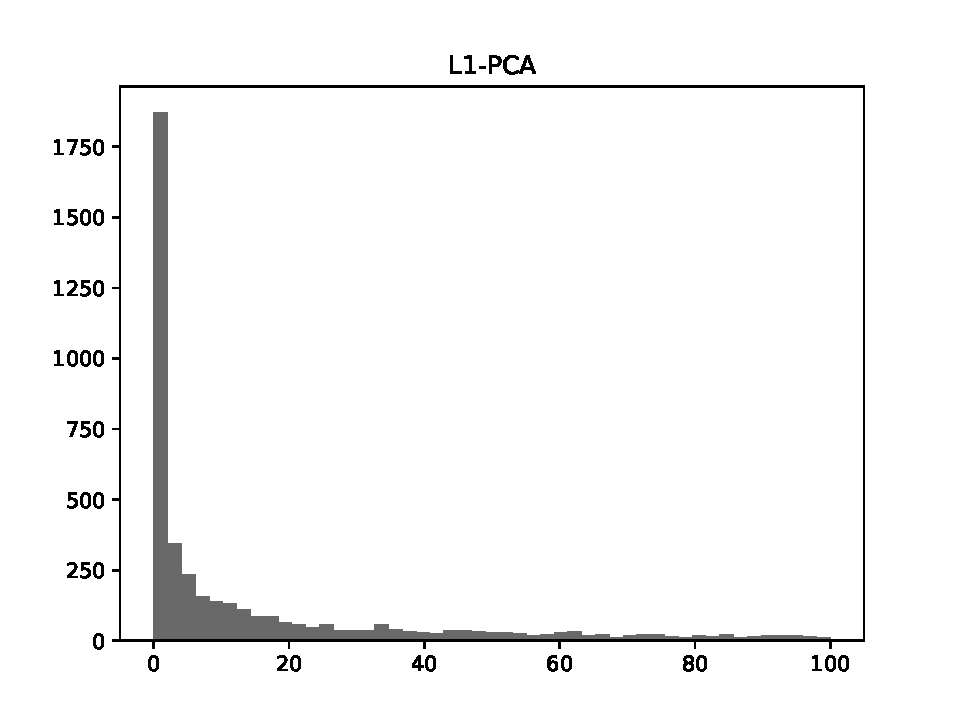
\includegraphics[width=4.9cm]{pics/lab1/l1-pca.pdf}
    \end{minipage}
    \begin{minipage}[t]{0.3\textwidth}
    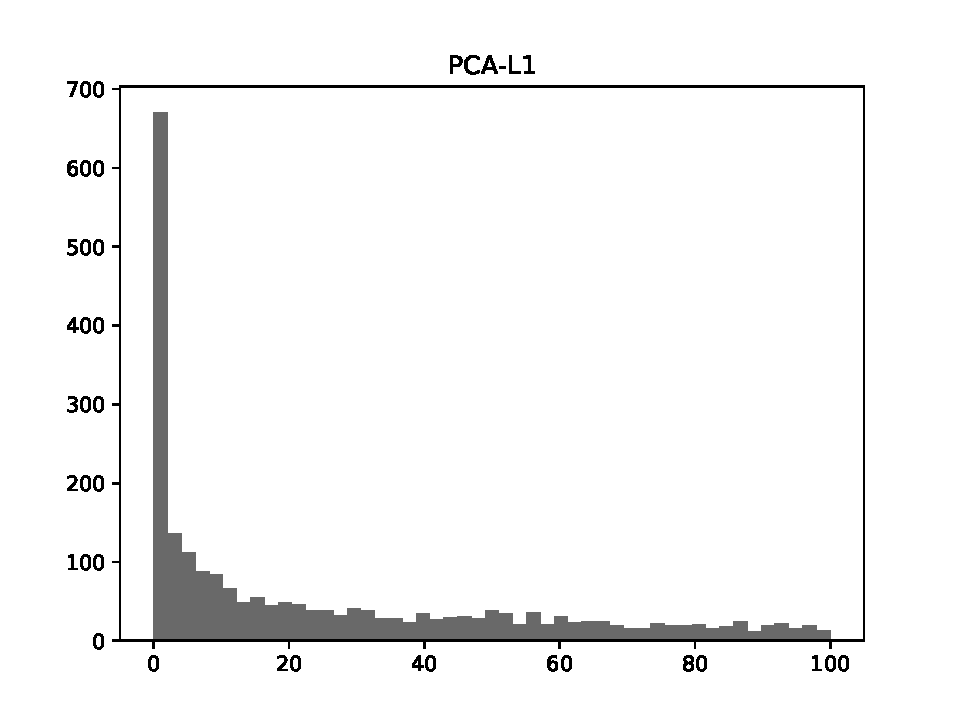
\includegraphics[width=4.9cm]{pics/lab1/pca-l1.pdf}
    \end{minipage}
    \begin{minipage}[t]{0.3\textwidth}
    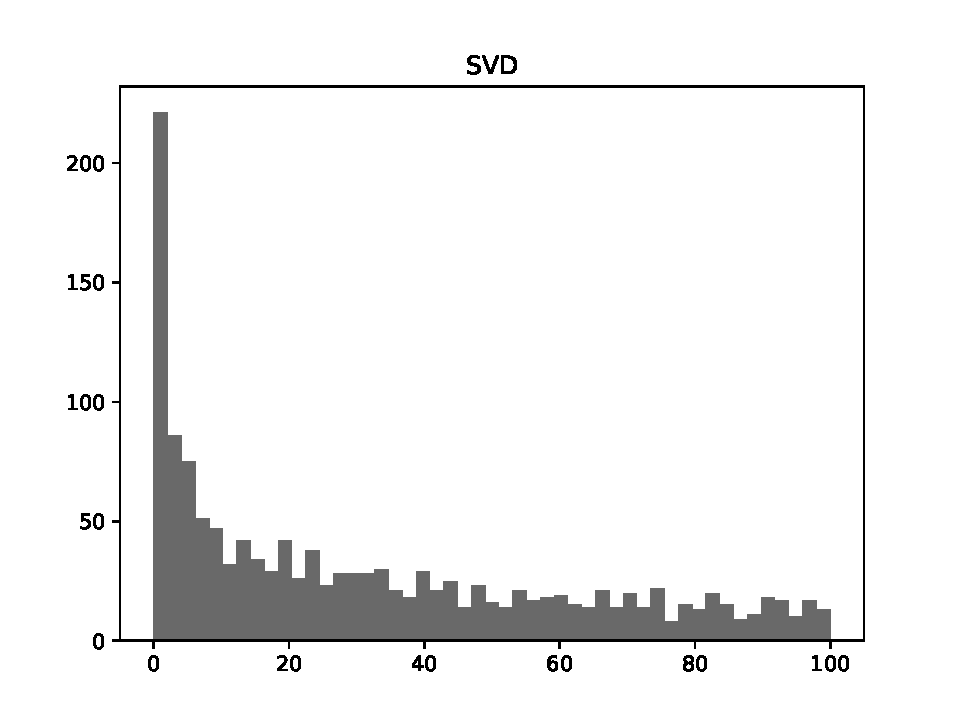
\includegraphics[width=4.9cm]{pics/lab1/svd.pdf}
    \end{minipage}
    \caption{重构残差对比图}
    \label{compare-con-error}
\end{figure}

注意到$L_1$-PCA方法相比PCA-$L_1$在重构误差分布上更加靠近零,这个现象也符合两种方法的理论出发点相符合,
另一个可能的原因是在执行算法4.2时并没有获得全局最优解。
另外可以看到两种$L_1$主成分分析面对含有大量离群值的数据的稳健性均远好于$L_2$主成分分析,
我们的结论是$P_4$同样可以作为稳健主成分分析的手段,适合处理带有大量离群值的数据。

需要注意的是由于$P_3$和$P_4$并不是一组对偶问题,它们求解获得的主成分是不同的。
\begin{figure}[H]
    \centering
    \begin{minipage}[t]{0.3\textwidth}
    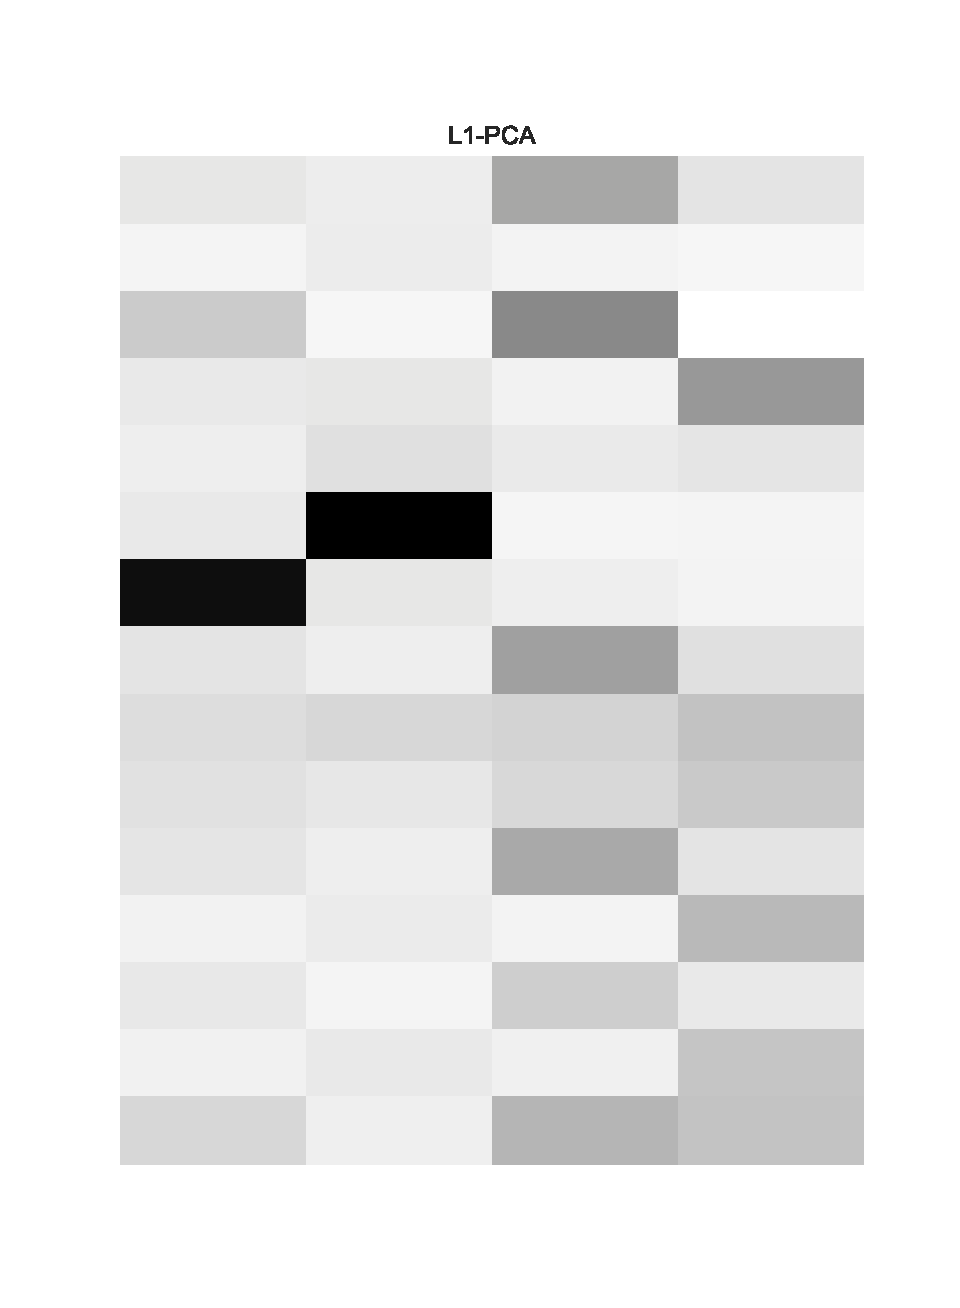
\includegraphics[width=4.9cm,height=8cm]{pics/lab1/l1-pca-rotated.pdf}
    \end{minipage}
    \begin{minipage}[t]{0.3\textwidth}
    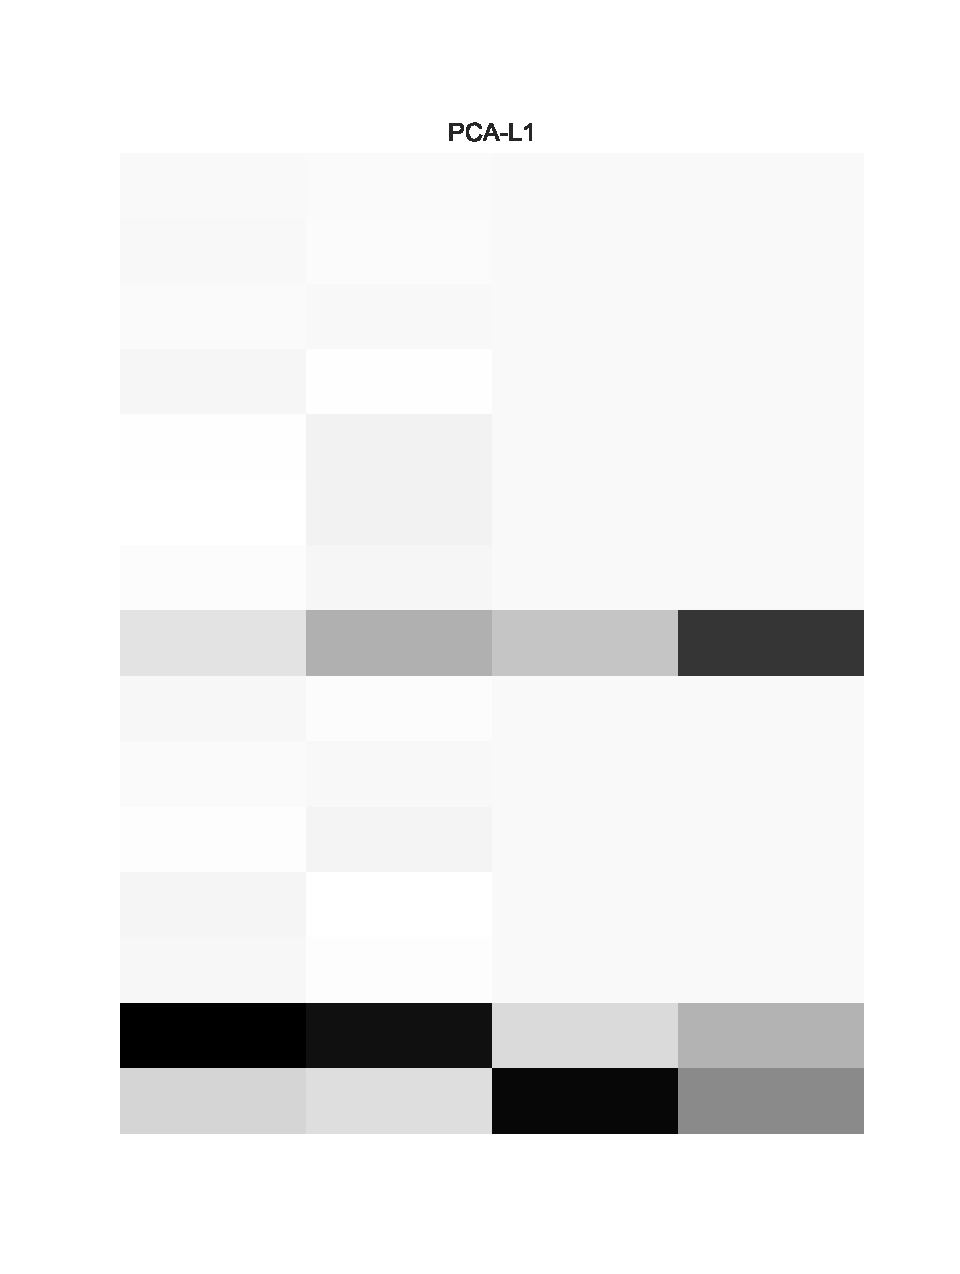
\includegraphics[width=4.9cm,height=8cm]{pics/lab1/pca-l1-rotated.pdf}
    \end{minipage}
    \begin{minipage}[t]{0.3\textwidth}
    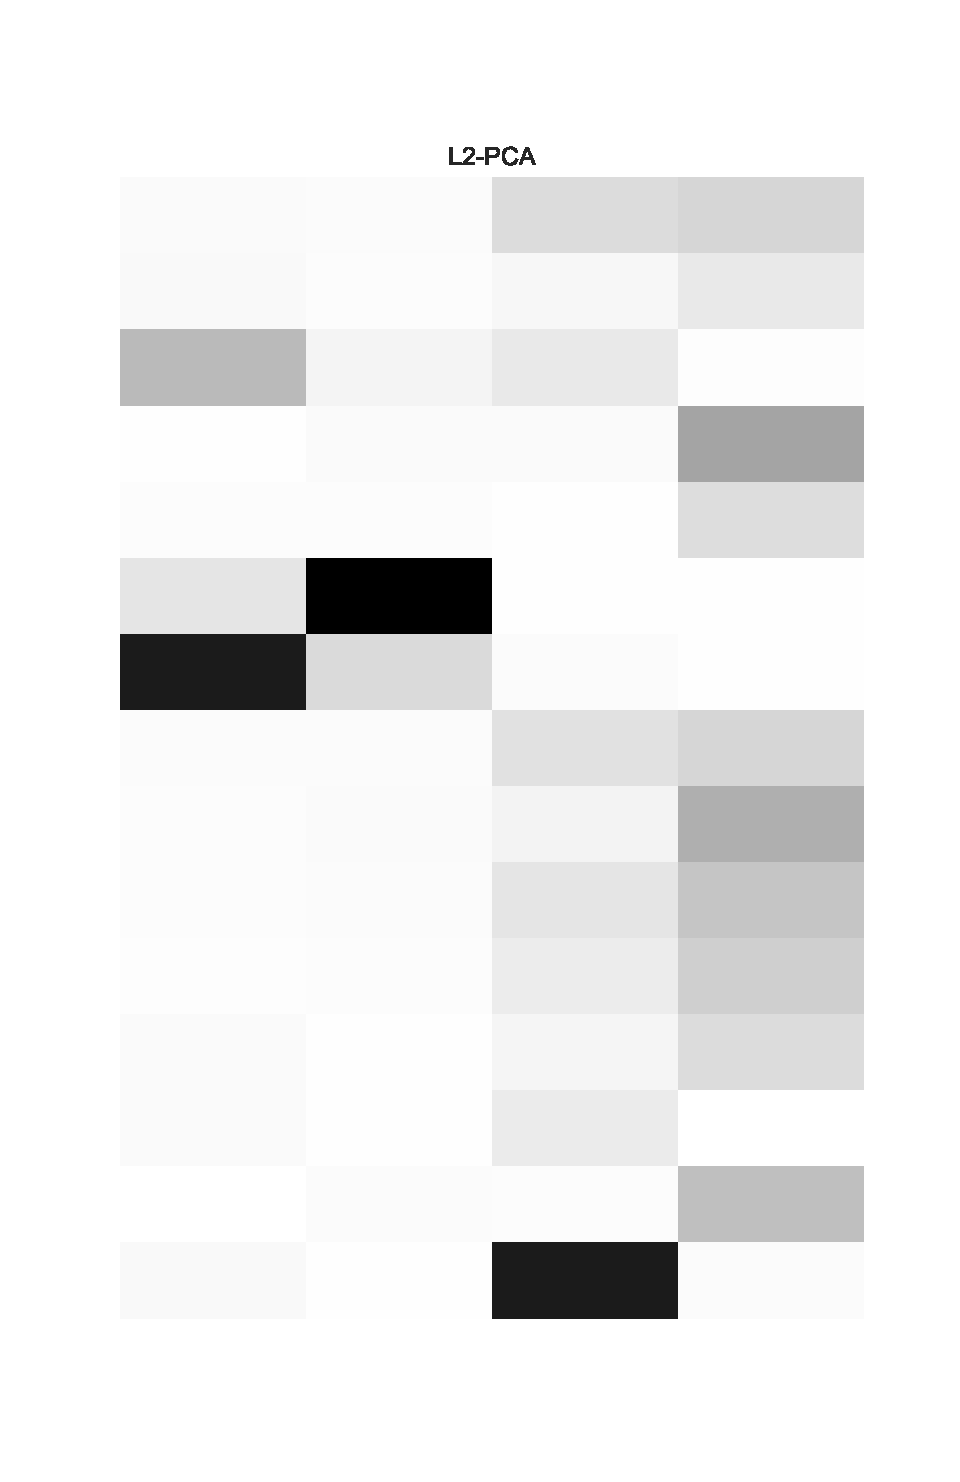
\includegraphics[width=4.9cm, height=8cm]{pics/lab1/l2-pca-rotated.pdf}
    \end{minipage}
    \caption{旋转后的因子载荷矩阵}
    \label{compare-rotate}
\end{figure}

图\ref{compare-rotate}中展示了同一组数据(模拟数据$m = 4, n = 15$)分别采用PCA-$L_1$、$L_1$-PCA以及$L_2$-PCA得到的因子载荷矩阵热力图。
为便于分析,我们已将因子载荷矩阵进行了最大方差旋转,可以看出三种不同的主成分分析方法得到的主成分是很不一样的。

前文已经通过实证研究发现,$L_1$-PCA估计得到的因子得分
在扩散指数模型中拥有良好的预测表现。
这里我们同样基于国内月度宏观经济数据对PCA-$L_1$进行测试,将得到的$L_1$因子得分
应用于扩散指数模型对部分指标进行经济预测。

我们列出一些在第\ref{chapter2}章中展示的经济指标预测情况,部分结果见表\ref{outcome4}至表\ref{outcome6}。

\begin{table}[H]
    \centering
    \small
    \caption{向前一个月预测结果}
    \label{outcome4}
    \begin{tabularx}{\textwidth}{lXXXXXX}
    \toprule
                 &  MSE(L1 PCA) &  MSE(PCA L1) &  MAE(L1 PCA) &  MAE(PCA L1) &  MPAE(L1 PCA) &  MPAE(PCA L1) \\ \midrule
    消费者满意指数     & 0.81            & 0.78        & 0.87            & 0.83        & 0.43             & 0.67         \\
    工业生产者出厂价格指数 & 0.70            & 0.83        & 0.75            & 0.92       & 0.96             & 0.90         \\
    货币供应量M2      & 0.76            & 1.01        & 0.90            & 1.00       & 0.45             & 0.92         \\
    固定资产投资总额  & 0.89            & 1.11        & 0.97            & 1.03        & 0.81             & 1.05         \\
    房地产开发投资总额 & 0.79            & 0.94        & 0.95            & 0.97        & 0.91             & 1.10         \\
    社会消费品零售总额 & 0.84            & 0.62        & 0.87            & 0.78        & 0.45             & 0.76         \\
    制造业采购经理指数    & 1.24            & 0.99        & 1.06            & 1.14        & 0.90             & 0.82         \\
    住宅新开工面积总数  & 0.89            & 1.20        & 0.85            & 1.12        & 0.45             & 1.19         \\
    股票流通市值     & 0.99            & 1.23        & 0.98            & 1.12        & 0.81             & 0.98         \\
    消费者信心指数     & 0.93            & 0.70        & 0.98            & 0.80        & 0.98             & 0.99         \\ \bottomrule
    \end{tabularx}
\end{table}

\begin{table}[H]
    \centering
    \small
    \caption{向前三个月预测结果}
    \label{outcome5}
    \begin{tabularx}{\textwidth}{lXXXXXX}
    \toprule
                 &  MSE(L1 PCA) &  MSE(PCA L1) &  MAE(L1 PCA) &  MAE(PCA L1) &  MPAE(L1 PCA) &  MPAE(PCA L1) \\ \midrule
                 消费者满意指数    & 0.85            & 1.16        & 0.95            & 1.22        & 1.32             & 0.78         \\
    工业生产者出厂价格指数& 0.98            & 0.88        & 0.97            & 0.93        & 0.93             & 0.97         \\
    货币供应量M2       & 1.08            & 0.59        & 1.05            & 0.71        & 0.66             & 0.70         \\
    固定资产投资总额  & 0.99            & 1.03        & 0.98            & 1.06       & 0.82             & 0.90         \\
    房地产开发投资总额 & 0.91            & 0.97        & 0.92            & 1.00       & 0.66             & 0.89         \\
    社会消费品零售总额 & 0.62            & 1.48        & 0.85            & 1.24        & 1.26             & 1.50        \\
    制造业采购经理指数    & 1.26            & 0.90        & 1.10            & 0.93        & 1.04             & 0.87         \\
    住宅新开工面积总数   & 0.81            & 0.75        & 1.12            & 0.89        & 1.04             & 0.90         \\
    股票流通市值   & 0.99            & 1.44        & 1.00            & 1.31        & 1.04             & 1.22         \\
    消费者信心指数    & 0.99            & 1.12        & 0.96            & 1.00        & 0.94             & 1.03         \\ \bottomrule
    \end{tabularx}
\end{table}

\begin{table}[H]\label{outcome3}
    \centering
    \small
    \caption{向前六个月预测结果}
    \label{outcome6}
    \begin{tabularx}{\textwidth}{lXXXXXX}
    \toprule
                 &  MSE(L1 PCA) &  MSE(PCA L1) &  MAE(L1 PCA) &  MAE(PCA L1) &  MPAE(L1 PCA) &  MPAE(PCA L1) \\ \midrule
                 消费者满意指数     & 0.91            & 1.00        & 0.93            & 1.00        & 0.68             & 0.99         \\
    工业生产者出厂价格指数 & 1.00            & 1.40        & 0.94            & 1.19        & 0.79             & 1.28         \\
    货币供应量M2      & 0.84            & 0.99        & 1.06            & 1.00        & 1.46             & 1.04         \\
    固定资产投资总额  & 0.88            & 0.69        & 0.94            & 0.73        & 0.93             & 0.85         \\
    房地产开发投资总额 & 0.90            & 0.58       & 0.91            & 0.67        & 0.73             & 0.79        \\
    社会消费品零售总额 & 0.64            & 1.36        & 0.79            & 1.14        & 1.30             & 1.45         \\
    制造业采购经理指数   & 1.46            & 1.20        & 1.20            & 1.09        & 1.45             & 1.42         \\
    住宅新开工面积总数  & 0.85            & 0.83        & 0.96            & 0.92        & 0.70             & 0.69        \\
    股票流通市值   & 0.98            & 1.20        & 1.01            & 1.16        & 1.28             & 0.97         \\
    消费者信心指数     & 0.99            & 1.07        & 0.98            & 1.00        & 0.97             & 0.87         \\ \bottomrule
    \end{tabularx}
\end{table}

从结果中可以看出,采用PCA-$L_1$估计得到的因子得分同样具有很好的预测表现。在向前一个月的预测中,其表现与$L_1$-PCA估计
得到的因子得分较为接近,都好于$L_2$主成分估计的因子得分。在向前一个季度与半年的预测中,两种$L_1$主成分分析
的预测表现都稍强于$L_2$主成分分析。

\subsection{本章小结}
本章进一步讨论了$L_1$范数主成分分析的求解算法问题。
首先我们结合上一章的研究内容,结合交替凸优化算法的特点,
对其涉及最小绝对值回归的步骤做出了改进。通过一个因子模型
数据的模拟实验,我们比较了改进后的算法的性能。由于实验平台
计算能力的限制,我们的实验结果稍显不够详尽。
然而实验结果已经能够发现,在对因子模型进行$L_1$主成分估计的
场合,我们对交替凸优化算法的改进尝试是有明显效果的。

另外针对$L_1$范数主成分分析的另一种求解思路,
我们也介绍了实现的经典算法。通过模拟实验和实证,
证明了两种$L_1$范数主成分分析的求解都具有很好的稳健性,
并且同样适用于扩散指数模型进行宏观经济预测。

